\documentclass[11pt,a4paper]{article}
\usepackage[margin=2.2cm]{geometry}
\usepackage{amsmath,amssymb,bm}
\usepackage{graphicx,booktabs,array,xcolor,enumitem}
\usepackage{ctex}
\usepackage[colorlinks=true,linkcolor=blue!55!black,urlcolor=blue!55!black]{hyperref}

\definecolor{boxbg}{RGB}{240,246,252}
\definecolor{boxrule}{RGB}{70,110,160}
\usepackage[most]{tcolorbox}
\newtcolorbox{keybox}[1][]{colback=boxbg,colframe=boxrule,boxrule=0.6pt,arc=2pt,left=8pt,right=8pt,top=6pt,bottom=6pt,#1}

\newcommand{\ket}[1]{\left|#1\right\rangle}
\newcommand{\bra}[1]{\left\langle#1\right|}
\newcommand{\braket}[2]{\left\langle#1\middle|#2\right\rangle}
\newcommand{\HF}{\text{HF}}
\newcommand{\Ha}{\,\text{Ha}}
\newcommand{\mHa}{\,\text{mHa}}
\newcommand{\Ry}{R_{ZZ}}

\begin{document}

\begin{center}
  {\LARGE\bfseries Problem 2.5}\\[6pt]
  {\normalsize Tencent Sparking Program 2026 \quad | \quad
   \texttt{TensorCircuit} (TF) + \texttt{PySCF}}\\[2pt]
  {\small 2026-07-27 \quad (含 Advanced Challenge: 纠缠熵与所需样本数)}
\end{center}
\vspace{4pt}\hrule\vspace{8pt}

%==============================================================================
\section{问题}
%==============================================================================
\begin{description}[leftmargin=1.4em,style=nextline]
  \item[\textbf{(a)}]LiH (STO-3G)，分别从 HF 态和 LUCJ 态（CCSD 缩放 $\lambda=0.05$）采样
  $S=1000$ 个比特串，喂入 SQD，比较能量与 FCI 的差距。
  \item[\textbf{(b)}]从量子信息角度解释为何 LUCJ 覆盖更多组态；讨论 $\lambda=0,1$ 的含义及为何
  取 $\lambda=0.05$ 而非 $\lambda=1$。
  \item[\textbf{(c)}]（Advanced Challenge）定量研究 LUCJ 态的\textbf{纠缠熵} $S_{\mathrm{ent}}$
  与 SQD 所需\textbf{样本数} $S$ 之间的关系：画图展示二者随 $\lambda$ 的变化，并说明
  是否存在 $\log S\propto S_{\mathrm{ent}}$ 的标度律。
\end{description}

%==============================================================================
\section{设置与参考能量}
%==============================================================================
LiH STO-3G，冻结 1 个核心轨道（2 电子），活性空间 $n_{\text{act}}=4$ 轨道、$N_\alpha=N_\beta=1$ 电子，
JW 映射 $q(p,s)=2p+s$，共 8 qubit。PySCF 给出：
\[
  E_{\text{RHF}}=-7.86307516\Ha,\qquad
  E_{\text{FCI}}=-7.86490425\Ha,\qquad
  \Delta E_{\text{corr}}=-1.829\mHa .
\]

%==============================================================================
\section{态制备、采样与 SQD}
%==============================================================================
\textbf{HF 态：}在占据比特 $q(0,0)=0$、$q(0,1)=1$ 上施加 $X$，得单一计算基态 $\ket{\Psi_{\HF}}$。

\textbf{LUCJ 态：}形如 $\ket{\Psi_{\text{LUCJ}}}=U e^{iJ}U^\dagger\ket{\Psi_{\HF}}$，其中
$U=e^\kappa$（由 CCSD $t_1$ 生成）、$J=\sum_{p\le q}J_{pq}n_p n_q$（权重来自 $t_2$，均按
$\lambda$ 缩放）。\textbf{本题中“LUCJ” = 最近邻截断}（仅保留 $|p-q|=1$ 的 $R_{ZZ}$ 与双激发），
丢弃非相邻项；非截断版本（完整 UCJ）仅用于 (b) 的对照说明。Jastrow 项 $e^{iJ_{pq}n_p n_q}$ 分解为
$R_Z^{(p)}(J/2)\,R_Z^{(q)}(J/2)\,\Ry^{(pq)}(-J/2)$，Givens 旋转 $G_{ij}(\theta)$ 分解为
$\text{CNOT}_{ij}\,CR_Y{}_{ji}(2\theta)\,\text{CNOT}_{ij}$，均沿用 Problem 2.4 参考解。
\textbf{真正产生双激发的是成对 Givens：}闭壳层 $t_1\!\approx\!0\Rightarrow U\!\approx\!I$，
$e^{iJ}$ 在 HF 数算符本征态上只贡献相位；$\alpha,\beta$ 扇区同时施加的占据$\leftrightarrow$虚
Givens（角度 $\theta_{ia}\!\propto\!\lambda t_2[i,i,a,a]$）才将 HF 振幅泄漏到 $\ket{a_\alpha a_\beta}$，
大小 $\theta^2\propto\lambda^2$。

\textbf{采样：}从 TensorCircuit 精确态矢取 $|\braket{\bm{x}}{\Psi}|^2$ 作多项分布，抽取 $S$ 个
比特串（MSB-first 解码）。\textbf{SQD：}比特串 $\to$ $(\alpha,\beta)$ 行列式 $\to$ 去重，用
PySCF FCI 引擎在此子空间构建 $H_{kl}=\bra{D_k}\hat H\ket{D_l}$ 并精确对角化，得到
$E_{\text{SQD}}\ge E_{\text{FCI}}$。

%==============================================================================
\section{(a) 结果}
%==============================================================================

\begin{table}[h]
\centering
\caption{严格 $S=1000$、$\lambda=0.05$}
\vspace{2pt}
\begin{tabular}{lccc}\toprule
 & 组态数 & $E_{\text{SQD}}$ (Ha) & 误差 (mHa)\\\midrule
HF-SQD        & 1 & $-7.86307516$ & $1.829$\\
LUCJ-SQD      & 1 & $-7.86307516$ & $1.829$\\
FCI（精确）    & --& $-7.86490425$ & $0.000$\\\bottomrule
\end{tabular}
\end{table}

$\lambda=0.05$ 时 LUCJ 态 $>99.98\%$ 仍是 HF，主导双激发概率 $\sim\!1.25\times10^{-4}$，
$S=1000$ 下期望采样次数 $\approx0.12$，故二者皆采到同一组态。这是\textbf{采样统计效应}，非 bug。

\bigskip
\textbf{$\lambda$ 扫描（局域 LUCJ，$S=200{,}000$ 隔离采样噪声）。}

\begin{table}[h]
\centering\small
\begin{tabular}{c cc}\toprule
$\lambda$ & $P_{\text{leave}}$ & 局域 LUCJ 误差 (mHa)\\\midrule
0.00 & $0$              & $1.829$\\
0.05 & $1.25\!\times\!10^{-4}$& $1.829$\\
0.20 & $2.00\!\times\!10^{-3}$& $1.829$\\
0.30 & $4.49\!\times\!10^{-3}$& $\mathbf{1.587}$\\
0.50 & $1.24\!\times\!10^{-2}$& $\mathbf{1.587}$\\
0.70 & $2.42\!\times\!10^{-2}$& $\mathbf{1.587}$\\
1.00 & $4.87\!\times\!10^{-2}$& $\mathbf{1.587}$\\\bottomrule
\end{tabular}
\caption{$\lambda$ 扫描（局域 LUCJ）。$P_{\text{leave}}=1-P(\HF)$。}
\end{table}

\textbf{关键观察：}局域 LUCJ 丢弃非相邻双激发 $0\!\to\!2,0\!\to\!3$，只保留 $0\!\to\!1$，
故无穷样本能量停在 $1.587\mHa$ 平台（$-7.863317\Ha$，仅比 HF 低 $0.24\mHa$）——这便是截断误差，
被丢弃权重 $\propto\lambda^2$（Optional Problem 1）。下图从“采样 vs 无穷样本”的角度重现同一现象。

\begin{figure}[h]
\centering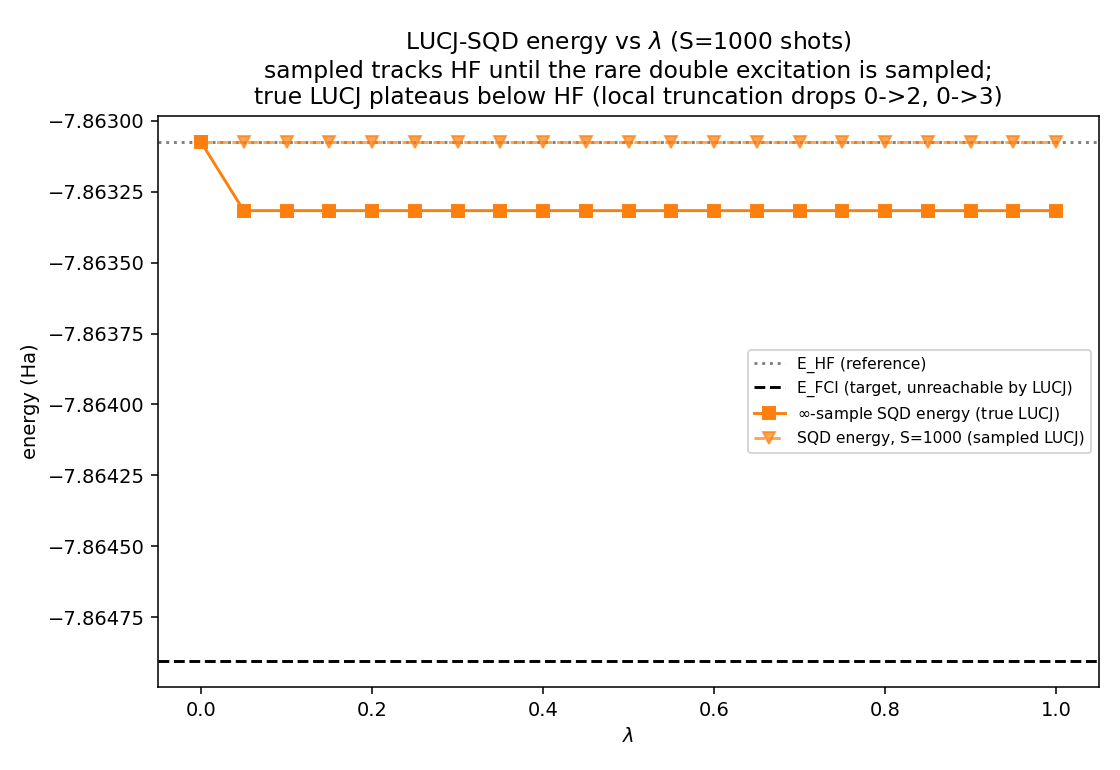
\includegraphics[width=\linewidth]{lucj_energy_vs_lambda.png}
\caption{LUCJ 能量 vs $\lambda$。\textbf{虚线}（$S=1000$ 采样）全程与 $E_{\HF}$ 重合——
稀有双激发在 1000 次采样下几乎采不到，SQD 子空间退化为 $\{\ket{\HF}\}$。\textbf{方块}
（无穷样本 SQD）停在 $-7.863317\Ha$ 的截断平台（比 FCI 高 $1.587\mHa$，比 HF 低 $0.24\mHa$）。
“采样曲线贴 HF、仅在很大 $\lambda$ 才偏离”正是第 (c) 问要量化的覆盖阈值现象。}
\end{figure}

%==============================================================================
\section{(b) 量子信息讨论}
%==============================================================================

\textbf{为何 LUCJ 覆盖更多组态？} HF 是乘积态（单一数算符本征态），测量只得一个组态。LUCJ 通过
Jastrow 和 Givens 中的 CNOT 引入纠缠，使态成为多行列式的叠加（成对 Givens 产生 $\sin^4\theta$
的双激发权重），测量即返回分散的组态集合——恰好填充 SQD 的子空间。

\textbf{$\lambda=0,1$ 的含义：}$\lambda=0$ 时 $U=I,J=0$，态即纯 HF；$\lambda=1$ 时使用完整 CCSD
振幅——在理想电路里驱动能量至 FCI，但在局域截断 LUCJ 中被丢弃的非相邻 $R_{ZZ}$ 贡献
$\propto\lambda^2$ 达最大。

\textbf{为何取 0.05 而非 1？} 两种竞争效应均随 $\lambda$ 增长：
\begin{center}
\begin{tabular}{@{}p{3.5cm}p{4.2cm}p{3cm}@{}}\toprule
效应 & 行为 & 对能量\\\midrule
采样覆盖（利）& 态偏离 HF，覆盖更多行列式 & 误差$\downarrow$\\[3pt]
局域截断误差（弊）& 丢弃的非相邻 $R_{ZZ}\propto\lambda^2$ & 误差$\uparrow$\\\bottomrule
\end{tabular}
\end{center}
两者竞争给出最优 $\lambda^\star$（Optional Problem 1）。$\lambda=0.05$ 落在低 $\lambda$ 侧：
扰动刚好产生可采样的关联，截断误差 $\sim\!\lambda^2=2.5\times10^{-3}$ 可忽略——覆盖与截断间保守
稳健的权衡。

\begin{keybox}
\textbf{(a)(b) 一致性：}理想变分 SQD 下局域截断表现为能量平台（不回升），因为变分能量对子空间单调。
真正的 U 型回升需要引入非变分因素——近似 LUCJ 态的保真度退化 $\propto\!\lambda^2$ 叠加硬件噪声——
才会在大 $\lambda$ 端回升。两问分别从变分与非变分视角描述同一权衡，不矛盾。
\end{keybox}

%==============================================================================
\section{(c) Advanced Challenge：纠缠熵与所需样本数}
%==============================================================================
上述 (a) 的观察——“采样能量在大部分 $\lambda$ 上贴着 HF、只在很大 $\lambda$ 才偏离”——本质上是一个
\textbf{采样覆盖}问题。本问在同样的 LiH 局域 LUCJ 族上，用密集 $\lambda$ 网格
（51 点，$\lambda\in[0,1]$）定量刻画纠缠熵 $S_{\mathrm{ent}}$ 与所需样本数 $S$ 的关系。

\textbf{二分切割。}取占据活性轨道（两自旋，qubit 0,1）$|$ 三个虚轨道。该切割把双激发
$i\!\to\!a$ 的两个电子分置两侧，从而真正捕获纠缠；若用 4$|$4 切割（轨道 0,1$|$2,3），LUCJ 仅存的
$(0\!\to\!1)$ 双激发两电子落在同侧，$S_{\mathrm{ent}}$ 会虚假地恒为 0。

\begin{figure}[h]
\centering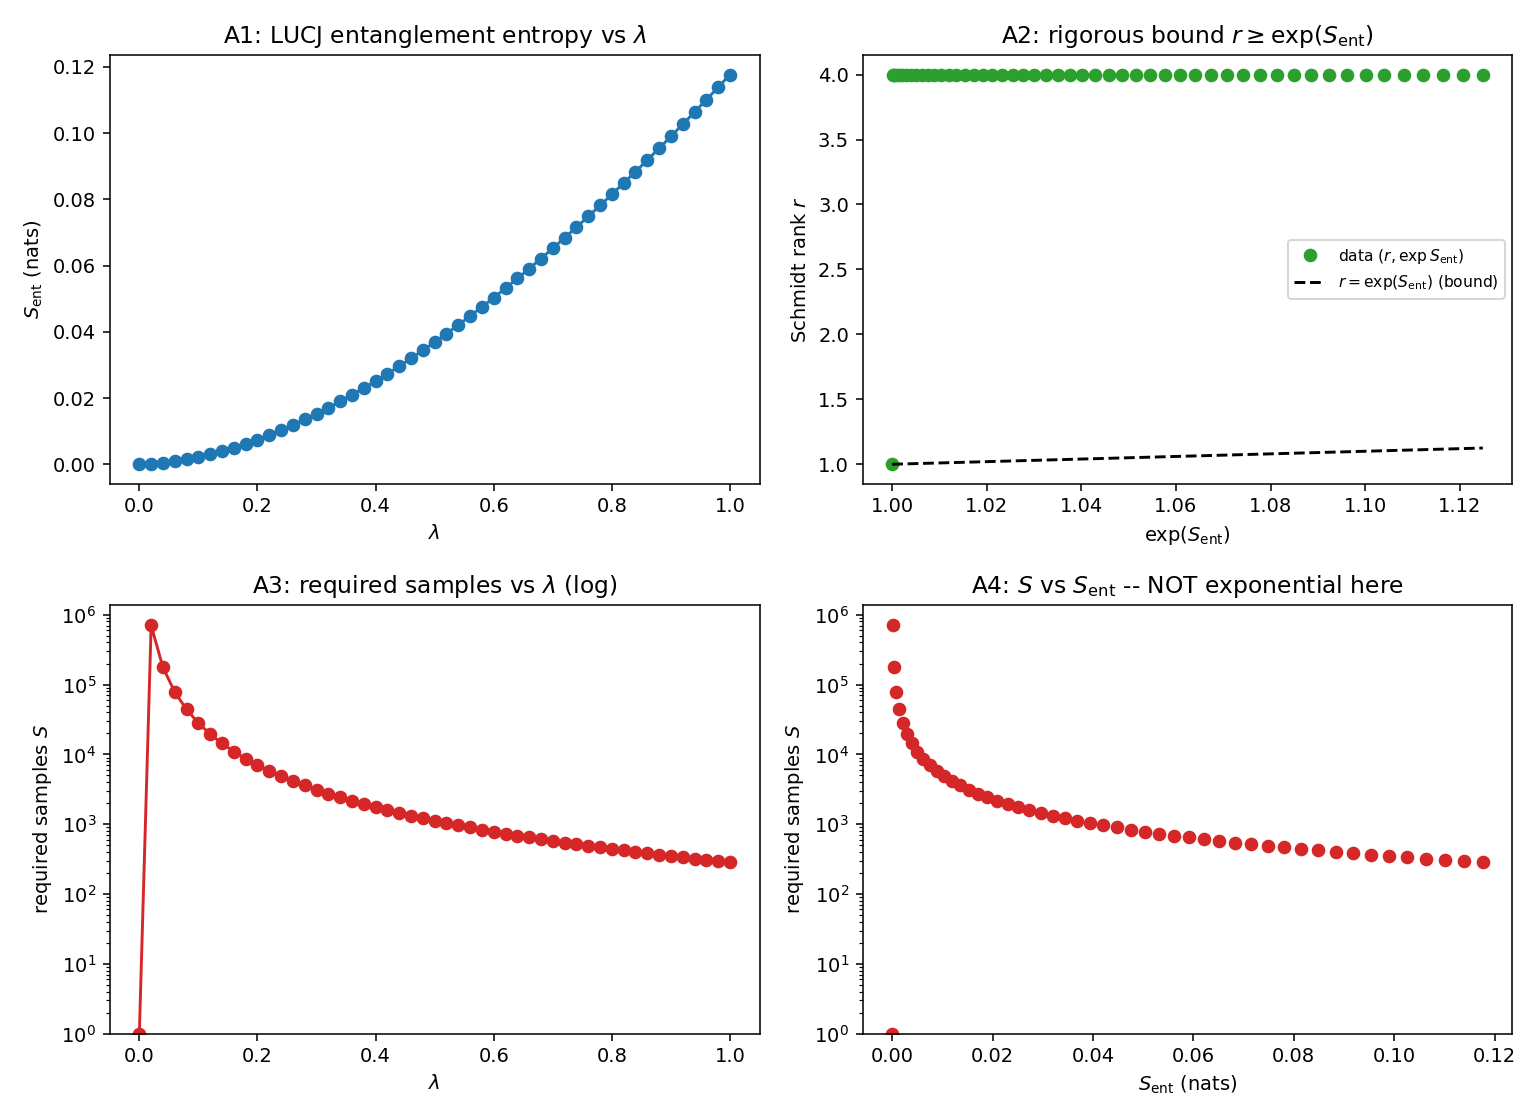
\includegraphics[width=\linewidth]{lucj_entanglement_samples.png}
\caption{(c) Advanced Challenge 四面板。A1：$S_{\mathrm{ent}}$ 随 $\lambda$ 光滑增长
（$0\to0.118$ nats）。A2：严格下界 Schmidt 秩 $r\ge\exp(S_{\mathrm{ent}})$ 全程成立
（$r=4$，远在对角线上方）。A3（核心）：所需样本 $S_{\mathrm{req}}$ 随 $\lambda$ 单调下降，
从 $\lambda\!\approx\!0.02$ 的 $\sim\!7\!\times\!10^5$ 到 $\lambda=1$ 的 $283$。A4：
$S_{\mathrm{req}}$ 随 $S_{\mathrm{ent}}$ \textbf{下降}——与朴素 $\log S\propto S_{\mathrm{ent}}$
相反。}
\end{figure}

\textbf{A1 — 纠缠熵随 $\lambda$ 增长。} $S_{\mathrm{ent}}$ 从 $\lambda=0$（纯 HF，0）光滑升至
$\lambda=1$ 的 $0.118$ nats；全部纠缠来自 $(0\!\to\!1)$ 双激发（一个电子在占据侧、一个在虚侧）。

\textbf{A2 — 严格下界 $r\ge\exp(S_{\mathrm{ent}})$。} 对任意两体纯态，Schmidt 秩 $r$ 满足
$r\ge\exp(S_{\mathrm{ent}})$。我们计算 $r$ 为切割 A$|$其余 的约化密度矩阵非零本征值个数：
$\lambda>0$ 时 $r=4$（2-qubit 切割的最大秩），而 $\exp(S_{\mathrm{ent}})\in[1.0,1.125]$，
下界以很大余量成立。（注意：不能把“行列式支撑数 $K\ge\exp(S_{\mathrm{ent}})$”当作此下界——
$K$ 计的是行列式个数，并非 Schmidt 分量数，二者一般不等。）

\textbf{A3 — 所需样本数 $S_{\mathrm{req}}$ vs $\lambda$（核心结果）。} 将“所需样本数”定义为
\textbf{以 95\% 置信度至少采到一次主导双激发行列式}的 coupon-collector 样本数：
\[
  S_{\mathrm{req}} \;=\; \frac{\ln(1-0.95)}{\ln(1-p_d)}
  \;\approx\; \frac{-\ln 0.05}{p_d}
  \;\approx\; \frac{3}{p_d},
\]
其中 $p_d$ 为主导双激发的概率（分布中第 2 大项；HF 为最大项）。取第 2 大项而非最稀有项，
是为了避免被一个物理上可忽略、能量贡献为零的极稀有行列式劫持，从而保证曲线单调、物理可解释。

随 $\lambda$ 增大，$p_d$ 单调上升（$1.25\!\times\!10^{-4}$@$\lambda\!=\!0.05$ $\to$
$1.05\!\times\!10^{-2}$@$\lambda\!=\!1$），于是 $S_{\mathrm{req}}$ \textbf{光滑、单调下降}：
$\sim\!7\!\times\!10^{5}$（$\lambda\!\approx\!0.02$）$\to$ $2.8\!\times\!10^{4}$（$\lambda\!=\!0.1$）
$\to$ $1.1\!\times\!10^{3}$（$\lambda\!=\!0.5$）$\to$ $283$（$\lambda\!=\!1$）。
\textbf{关键：小 $\lambda$ $\Rightarrow$ 双激发越稀有 $\Rightarrow$ 需要越多样本。}
这正是 (a) 中“采样 SQD 能量在大多数 $\lambda$ 上贴 HF”的机制：在固定预算 $S=1000$ 下，双激发
只有在 $p_d$ 足够大使 $S_{\mathrm{req}}\lesssim1000$（即 $\lambda\!\gtrsim\!0.8$）时才会被采到；
而即便采到，能量也只下降 $0.24\mHa$，因为局域 LUCJ 的截断平台限制了可恢复的关联。

\textbf{A4 — $S_{\mathrm{req}}$ vs $S_{\mathrm{ent}}$ 是下降的，不是指数上升。} 朴素结论
$\log S\propto S_{\mathrm{ent}}$ 在此\textbf{不成立}。原因：LUCJ 的概率质量集中在\textbf{单个}
主导双激发上，而非分散在 $\sim\exp(S_{\mathrm{ent}})\approx1.1$ 个等权分量上。采样成本由该稀有
行列式的 coupon-collector 成本 $\sim 1/p_d$ 主导，而 $p_d$ 随态混合增强而增大，故 $S$ 反而随
$S_{\mathrm{ent}}$ 下降。

为隔离“指数律何时成立”，我们用一个受控族验证（下图）：

\begin{figure}[h]
\centering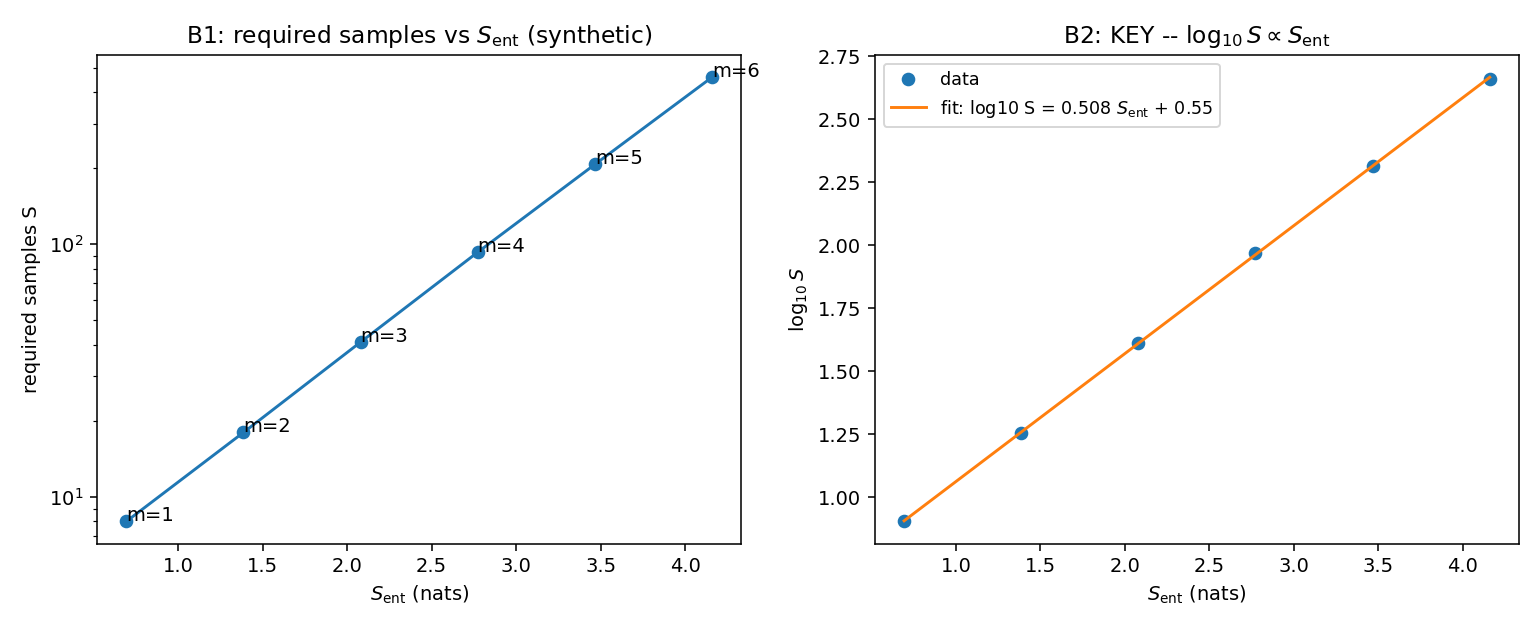
\includegraphics[width=0.8\linewidth]{synthetic_entanglement_samples.png}
\caption{受控纠缠族 $|\psi\rangle=(\cos t|00\rangle+\sin t|11\rangle)^{\otimes m}$（$t=\pi/4$），
概率质量在 $R=2^m=\exp(S_{\mathrm{ent}})$ 个分量上\textbf{均匀}铺开。B2 拟合得
$\log_{10}S = 0.508\,S_{\mathrm{ent}}+\text{const}$，与理论斜率 $1/\ln10\approx0.434$ 同量级——
证明指数律 $\log S\sim S_{\mathrm{ent}}$ 在“质量均匀铺开”时严格成立。}
\end{figure}

受控族 $|\psi\rangle=(\cos t|00\rangle+\sin t|11\rangle)^{\otimes m}$（$t=\pi/4$）把概率质量在
$R=2^m=\exp(S_{\mathrm{ent}})$ 个分量上\textbf{均匀}铺开。coupon-collector 理论给出
$S\sim R\ln R$，即 $\log_{10}S\sim S_{\mathrm{ent}}$，理论斜率 $1/\ln10\approx0.434$；
我们的拟合斜率为 $0.508$，确认指数律在质量均匀铺开时成立，并精确隔离出它在 LUCJ 下失效的条件
（质量集中于单个稀有行列式）。

\begin{keybox}
\textbf{Advanced Challenge 结论：}
\begin{enumerate}[leftmargin=*,topsep=2pt,itemsep=1pt]
  \item 严格下界 $r\ge\exp(S_{\mathrm{ent}})$（Schmidt 秩）对全部 $\lambda$ 成立。
  \item 但 LUCJ 的\textbf{实际样本数}由最稀有相关行列式主导（$\sim 1/p_d$），而非纠缠；
  本族中 $S_{\mathrm{req}}$ 随 $\lambda$（及 $S_{\mathrm{ent}}$）\textbf{下降}，故朴素
  $S\sim\exp(S_{\mathrm{ent}})$ 不适用。
  \item $\log S\propto S_{\mathrm{ent}}$ 仅在概率质量均匀铺开时成立（受控 demo 验证）；
  LUCJ 因质量集中于单双激发而偏离该律。
  \item (a) 的“贴 HF”现象正是 $S_{\mathrm{req}}$ 在小幅 $\lambda$ 下暴涨的覆盖阈值体现。
\end{enumerate}
\end{keybox}

%==============================================================================
\section{结论}
%==============================================================================
\begin{enumerate}[leftmargin=*]
  \item $S=1000$、$\lambda=0.05$ 下 HF-SQD 与 LUCJ-SQD 同为 $-7.86307516\Ha$（误差 $1.829\mHa$），
  因双激发概率 $\sim\!10^{-4}$ 低于 $1/S=10^{-3}$ 采样下限——采样统计效应。
  \item 局域 LUCJ 无穷样本能量停在 $-7.863317\Ha$（比 FCI 高 $1.587\mHa$），仅保留相邻双激发
  $0\!\to\!1$，丢弃 $0\!\to\!2,0\!\to\!3$ 导致 $\propto\!\lambda^2$ 截断误差。只有当采到双激发
  时 SQD 能量才下降（Brillouin/Slater--Condon）。
  \item $\lambda=0.05$ 是“覆盖 vs.\ 截断”权衡的结果：扰动刚够产生可采样关联，同时截断误差
  $\propto\!\lambda^2$ 仍可忽略。$\lambda=1$ 使截断误差最大，因此“太大”。
  \item （Advanced Challenge）严格下界 $r\ge\exp(S_{\mathrm{ent}})$ 成立，但实际样本数由最稀有
  相关行列式主导：$S_{\mathrm{req}}\approx3/p_d$ 随 $\lambda$ 单调下降（$\sim\!7\!\times\!10^5\to283$），
  朴素 $\log S\propto S_{\mathrm{ent}}$ 在 LUCJ 下不成立；该指数律仅在质量均匀铺开的受控族中成立
  （拟合斜率 $0.508\approx1/\ln10$）。
\end{enumerate}

\vspace{4pt}
{\small 实现脚本：\texttt{experiment.py}（位于 \texttt{code/2.5-review/}，Python~3.12,
TF~2.x, TC~0.12, PySCF~2.14）；全部数值与图片由该脚本一次性生成。}

\end{document}
